%%%%%%%%%%%%%%%%%%%%%%%%%%%%%%%%%%%%%%%%%%%%%%%%%%%
\begin{frame}
  \begin{center}
    {\Large Recurrent Neural Network (RNN)}
  \end{center}
\end{frame}


%%%%%%%%%%%%%%%%%%%%%%%%%%%%%%%%%%%%%%%%%%%%%%%%%%%
\begin{frame}[fragile] \frametitle{Sequences}

\begin{itemize}
\item Need to predict when the ball would be in the next moment?
\item Scenario 1: no info of previous state is given. Answer: random state.
\item Scenario 2: some info of previous state is given. Answer: possible to fit trajectory and predict.
\item Another example: On mobile, while typing sms you get some predictive suggestions !!!
\end{itemize}

\begin{center}
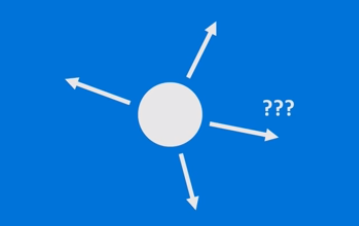
\includegraphics[width=0.3\linewidth,keepaspectratio]{rnn44}

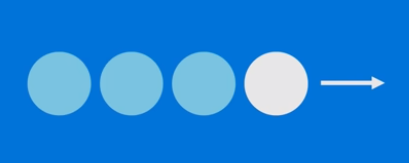
\includegraphics[width=0.3\linewidth,keepaspectratio]{rnn45}

\end{center}

{\tiny (Ref: Recurrent Neural Network - Ava Soleimany, January 2020 )}

\end{frame}


%%%%%%%%%%%%%%%%%%%%%%%%%%%%%%%%%%%%%%%%%%%%%%%%%%%
\begin{frame}[fragile] \frametitle{Recap: NN types: ANN, CNN, RNN}

\begin{itemize}
\item In ANN, columns are independent of each other. None of the neighbor information is used. Shuffling columns does not have any effect on the model/results.
\item In CNN, spatial (not `special') column-neighbors are used to form features, which help in discerning the categories in the classification.
\item In RNN, temporal (no, `temporary') neighbors/column-wise are used to form features, which help in predictions.
\end{itemize}

\end{frame}






%%%%%%%%%%%%%%%%%%%%%%%%%%%%%%%%%%%%%%%%%%%%%%%%%%%
\begin{frame}[fragile] \frametitle{So, Why RNN?}

\begin{itemize}
% \item Each sample (row) is independent or unlinked to other samples (rows)
% \item Weights are adjusted (optimized) have overall least Loss.
\item Problem is: ANNs do not have memory. Meaning, any bearing to the previous samples.
\item The model does not care about what came before.
\item Thats not useful in case of Sequences or Time Series. Here, past is useful in deciding the present and the future.
\item Solution: RNN
\end{itemize}


\end{frame}


%%%%%%%%%%%%%%%%%%%%%%%%%%%%%%%%%%%%%%%%%%%%%%%%%%%
\begin{frame}[fragile] \frametitle{Background}

\begin{itemize}
\item By Elman in 1990.
\item Proposed to have input layer, hidden ayer, context layer along with recurrent feedback.
\end{itemize}

\begin{center}
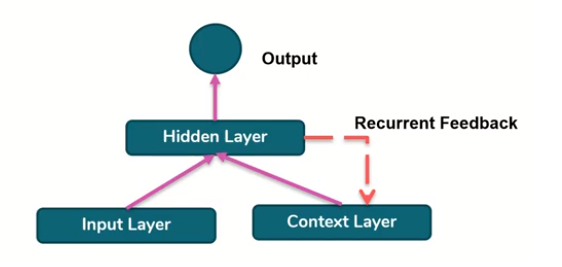
\includegraphics[width=0.8\linewidth,keepaspectratio]{rnn43}
\end{center}

{\tiny (Ref: Simple RNN Explained - Shriram Vasudevan)}

\end{frame}

%%%%%%%%%%%%%%%%%%%%%%%%%%%%%%%%%%%%%%%%%%%%%%%%%%%
\begin{frame}
  \begin{center}
    {\Large Toy Example}
		
		{\tiny (Ref: Luis Serrano)}
  \end{center}
\end{frame}

%%%%%%%%%%%%%%%%%%%%%%%%%%%%%%%%%%%%%%%%%%%%%%%%%%%
\begin{frame}[fragile] \frametitle{Toy Example: Scenario I: Cook}
An ideal roommate who cooks:
\begin{itemize}
\item Can cook 3 dishes: Apple Pie, Burger, Chicken
\item Dish depends on the outside weather (only Sunny or Rainy)
\begin{itemize}
\item Sunny: Apple Pie
\item Rainy: Burger
\end{itemize}
\end{itemize}
This can be easily modeled as Neural network with known inputs and outputs.


\begin{center}
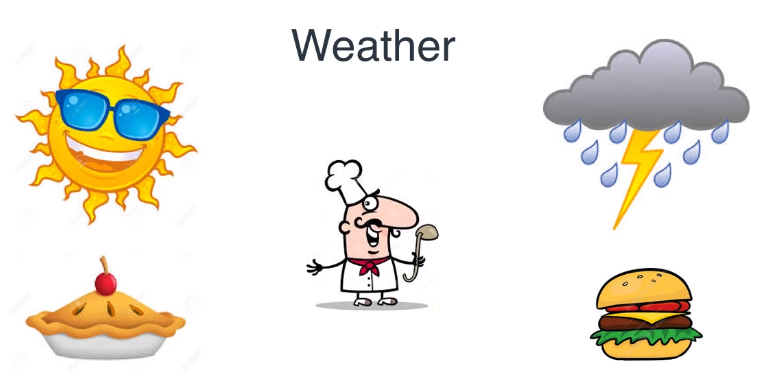
\includegraphics[width=0.8\linewidth,keepaspectratio]{rnn39}
\end{center}



\end{frame}

%%%%%%%%%%%%%%%%%%%%%%%%%%%%%%%%%%%%%%%%%%%%%%%%%%%
\begin{frame}[fragile] \frametitle{Toy Example: Scenario I}
Lets model food and weather as one-hot encoding vectors
\begin{center}
\includegraphics[width=\linewidth,keepaspectratio]{rnn6}
\end{center}
Network takes weather vector in and outputs food vector
\end{frame}

%%%%%%%%%%%%%%%%%%%%%%%%%%%%%%%%%%%%%%%%%%%%%%%%%%%
\begin{frame}[fragile] \frametitle{Toy Example: Scenario I}
\begin{itemize}
\item This Neural Network is represented by a matrix (3x2)g
\item Individual weather vector when post multiplies this matrix, resultant 3x1 vector represents food
\item For Sunny, you get Apple Pie
\item For Rainy, you get Burger.
\end{itemize}
\begin{center}
\includegraphics[width=\linewidth,keepaspectratio]{rnn7}
\end{center}
\end{frame}

%%%%%%%%%%%%%%%%%%%%%%%%%%%%%%%%%%%%%%%%%%%%%%%%%%%
\begin{frame}[fragile] \frametitle{Toy Example: Scenario I}
\begin{itemize}
\item Matrix can be seen as network as well.
\item First node emits 3 rays, each to each output node: 1, 0, 1. This is nothing but first column of the matrix
\item Second node emits 3 rays, each to each output node: 0, 1, 0. This is nothing but second column of the matrix
\item Input weather vector values are put into input nodes, multiplication happens and then output values are generated.
\end{itemize}
\begin{center}
\includegraphics[width=0.8\linewidth,keepaspectratio]{rnn8}
\end{center}
\end{frame}

%%%%%%%%%%%%%%%%%%%%%%%%%%%%%%%%%%%%%%%%%%%%%%%%%%%
\begin{frame}[fragile] \frametitle{Toy Example: Scenario II}

\begin{itemize}
\item Same roommate, but instead of weather he decides the dish based on previous day.
\item One day Apple Pie, next Burger, next Chicken.
\end{itemize}
\begin{center}
\includegraphics[width=\linewidth,keepaspectratio]{rnn9}
\end{center}
\end{frame}

%%%%%%%%%%%%%%%%%%%%%%%%%%%%%%%%%%%%%%%%%%%%%%%%%%%
\begin{frame}[fragile] \frametitle{Toy Example: Scenario II}

\begin{itemize}
% \item This can not be modelled using previously seen normal Neural network, its called Recurrent Neural Network (RNN)
\item There is no Weather input, but previous day's output is its input. Shown as loop.
\item This is Time Series, like stock prices.
\end{itemize}
\begin{center}
\includegraphics[width=0.8\linewidth,keepaspectratio]{rnn10}
\end{center}
\end{frame}


%%%%%%%%%%%%%%%%%%%%%%%%%%%%%%%%%%%%%%%%%%%%%%%%%%%
\begin{frame}[fragile] \frametitle{Toy Example: Scenario II}
As a network:
\begin{itemize}
\item 3 inputs, 3 outputs
\item Both representing food
\item Its basically looping back. So, its Recurrent.
\end{itemize}
\begin{center}
\includegraphics[width=0.5\linewidth,keepaspectratio]{rnn11}
\end{center}
\end{frame}

%%%%%%%%%%%%%%%%%%%%%%%%%%%%%%%%%%%%%%%%%%%%%%%%%%%
\begin{frame}[fragile] \frametitle{Toy Example: Scenario III}
\begin{itemize}
\item Same roommate, but now the rules of cooking are dependent on both, weather as well as previous day dish
\item If Sunny, he goes out, has fun, no cooking, so dish is leftover, same as yesterday
\item If Rainy, he is at home, next dish on the sequence.
\item Below, for Tuesday, it's Sunny weather is shown under Monday (just for illustration) as input
\item So inputs are Weathers, and also the predicted output of last day ie Food.
\end{itemize}
\begin{center}
\includegraphics[width=0.8\linewidth,keepaspectratio]{rnn12}
\end{center}
\end{frame}

%%%%%%%%%%%%%%%%%%%%%%%%%%%%%%%%%%%%%%%%%%%%%%%%%%%
\begin{frame}[fragile] \frametitle{Toy Example: Scenario III}
Input Vectors
\begin{center}
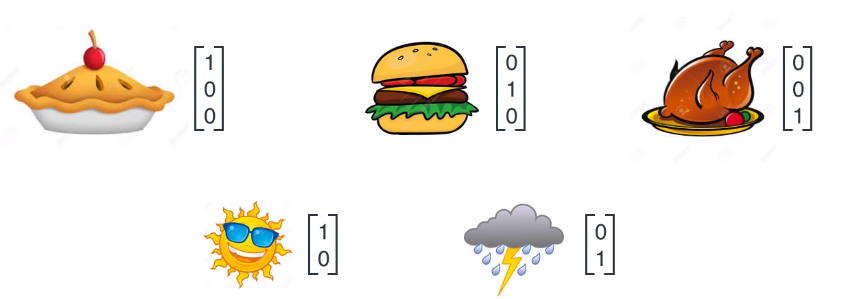
\includegraphics[width=0.8\linewidth,keepaspectratio]{rnn40}
\end{center}

Weight Matrices
\begin{center}
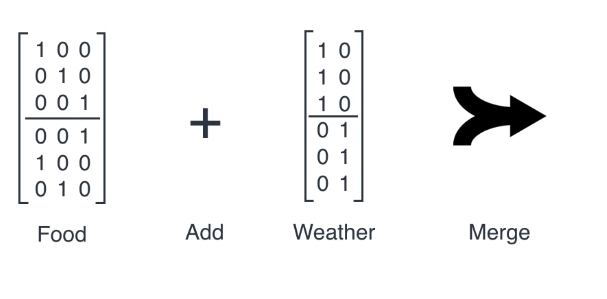
\includegraphics[width=0.6\linewidth,keepaspectratio]{rnn41}
\end{center}

They are divided into two portions, just to model two outputs. One for same day (can you see Identity matrix on top food portion) and another for the next day prediction.

\end{frame}


%%%%%%%%%%%%%%%%%%%%%%%%%%%%%%%%%%%%%%%%%%%%%%%%%%%
\begin{frame}[fragile] \frametitle{Toy Example: Scenario III}
Food Matrix
\begin{itemize}
\item Food matrix artificially cut into two
\item Top represents Sunny, bottom as Rainy
\item Apple Pie comes in, top results in Apple Pie as TODAY's food (same), bottom results in next dish, ToMORROW's food.
\item Nothing about Weather as of now.
\end{itemize}
\begin{center}
\includegraphics[width=0.8\linewidth,keepaspectratio]{rnn13}
\end{center}
\end{frame}

%%%%%%%%%%%%%%%%%%%%%%%%%%%%%%%%%%%%%%%%%%%%%%%%%%%
\begin{frame}[fragile] \frametitle{Toy Example: Scenario III}
Weather Matrix
\begin{itemize}
\item Top results are all 1's. Same as Today, Sunny as 1 represents Sunny, 0 Rainy.
\item Bottom result are all 0's. For Next day.
\item Weather matrix tells, if he as to cook TODAY's food or TOMORROW's food. As the bottom results are all 1's, or YES's.
\end{itemize}
\begin{center}
\includegraphics[width=0.8\linewidth,keepaspectratio]{rnn14}
\end{center}
\end{frame}

%%%%%%%%%%%%%%%%%%%%%%%%%%%%%%%%%%%%%%%%%%%%%%%%%%%
\begin{frame}[fragile] \frametitle{Toy Example: Scenario III}
\begin{itemize}
\item Combining two matrices should give clear signal on what to cook.
\item Food Matrix: Whats the food for today? Whats for tomorrow?
\item Weather Matrix: Should I cook today? or tomorrow?
\end{itemize}
\begin{center}
\includegraphics[width=0.8\linewidth,keepaspectratio]{rnn15}
\end{center}
\end{frame}


%%%%%%%%%%%%%%%%%%%%%%%%%%%%%%%%%%%%%%%%%%%%%%%%%%%
\begin{frame}[fragile] \frametitle{Toy Example: Scenario III}
Testing
\begin{itemize}
\item Say, we had Apple Pie yesterday and its rainy today
\item Food Matrix is computed and added to Weather Matrix
\end{itemize}
\begin{center}
\includegraphics[width=0.8\linewidth,keepaspectratio]{rnn16}
\end{center}
\end{frame}

%%%%%%%%%%%%%%%%%%%%%%%%%%%%%%%%%%%%%%%%%%%%%%%%%%%
\begin{frame}[fragile] \frametitle{Toy Example: Scenario III}
Merge
\begin{itemize}
\item We apply non linear function that takes input of the combined results
\item Maps it to uniform one-hot like result.
\item It make the LARGEST as 1, else all to 0
\item Add sub-components  and produces the result
\end{itemize}
\begin{center}
\includegraphics[width=0.8\linewidth,keepaspectratio]{rnn17}
\end{center}
\end{frame}

%%%%%%%%%%%%%%%%%%%%%%%%%%%%%%%%%%%%%%%%%%%%%%%%%%%
\begin{frame}[fragile] \frametitle{Toy Example: Scenario III}
Summary (shown arrows are 1)
\begin{center}
\includegraphics[width=\linewidth,keepaspectratio]{rnn18}
\end{center}
\end{frame}

%%%%%%%%%%%%%%%%%%%%%%%%%%%%%%%%%%%%%%%%%%%%%%%%%%%
\begin{frame}[fragile] \frametitle{Toy Example: Scenario III}
Recurrent
\begin{center}
\includegraphics[width=\linewidth,keepaspectratio]{rnn19}
\end{center}
\end{frame}

% %%%%%%%%%%%%%%%%%%%%%%%%%%%%%%%%%%%%%%%%%%%%%%%%%%%
% \begin{frame}[fragile] \frametitle{Toy Example: Scenario IV: Summary}
% \begin{itemize}
% \item We can group together inputs and outputs.
% \item Two inputs: yesterday's predictions and yesterday's dish
% \item One output: today's prediction
% \end{itemize}
% \begin{center}
% \includegraphics[width=0.8\linewidth,keepaspectratio]{rnn20}
% \end{center}
% \end{frame}

% %%%%%%%%%%%%%%%%%%%%%%%%%%%%%%%%%%%%%%%%%%%%%%%%%%%
% \begin{frame}[fragile] \frametitle{Toy Example: Scenario IV: Summary}
% \begin{itemize}
% \item Prediction is recycled as input
% \item The dotted line, holds it to be used today
% \end{itemize}
% \begin{center}
% \includegraphics[width=0.8\linewidth,keepaspectratio]{rnn21}
% \end{center}
% \end{frame}

% %%%%%%%%%%%%%%%%%%%%%%%%%%%%%%%%%%%%%%%%%%%%%%%%%%%
% \begin{frame}[fragile] \frametitle{Toy Example: Scenario IV: Summary}
% \begin{itemize}
% \item So, even if we missed few time steps in between, 
% \item We can play the actions forward from the known past time
% \end{itemize}
% \begin{center}
% \includegraphics[width=0.8\linewidth,keepaspectratio]{rnn22}
% \end{center}
% \end{frame}


%%%%%%%%%%%%%%%%%%%%%%%%%%%%%%%%%%%%%%%%%%%%%%%%%%%
\begin{frame}
  \begin{center}
    {\Large Theory of RNN}
  \end{center}
\end{frame}

%%%%%%%%%%%%%%%%%%%%%%%%%%%%%%%%%%%%%%%%%%%%%%%%%%%
\begin{frame}[fragile] \frametitle{What is RNN?}
A Neural network with a memory-state is added to the neurons. 
\begin{itemize}
\item When data is sequential
\item ANN: model produces the output by multiplying the input with the weight and the activation function
\item RNN: output is sent back to itself and this, along with the new input is used to calculate the new output.
% \item Next depends on previous + extra input
\item The network is called 'recurrent' because it performs the same operation in each timestep.
\item Example: Stock Predictions, Language Model (next word prediction), etc.
\end{itemize}


\begin{center}
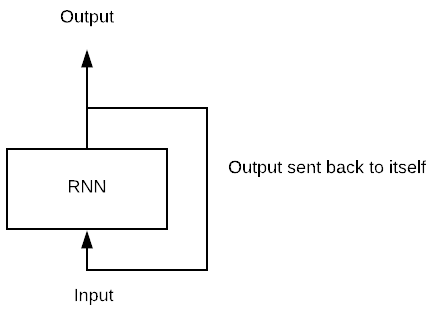
\includegraphics[width=0.3\linewidth,keepaspectratio]{rnn29}
\end{center}
\end{frame}


%%%%%%%%%%%%%%%%%%%%%%%%%%%%%%%%%%%%%%%%%%%%%%%%%%%
\begin{frame}[fragile] \frametitle{What is RNN?}
When:
\begin{itemize}
\item Order is important
\item Variable length
\item Sequential data
\item Each item is processed in context
\end{itemize}

\end{frame}


%%%%%%%%%%%%%%%%%%%%%%%%%%%%%%%%%%%%%%%%%%%%%%%%%%%
\begin{frame}[fragile] \frametitle{What is RNN?}
Usage of RNN layer:
\begin{itemize}
\item Input data points (X) one at a time.
% \item X is of size [ batch size, number of steps, number of dimensions]
% \item batch size: window of inputs data points, at once
\item Simple cell is just one node and an activation function, thats it.
\item GRU (Gated Recurrent Units) and LSTM (Long Short Term Memory) are two other types of RNN cells.
\item RNN layer will process sequential data. Output is flattened vector
\item Dense Layer is normal ANN, for prediction or classification (Y)
\end{itemize}


\begin{center}
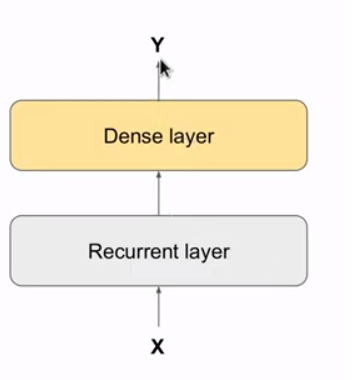
\includegraphics[width=0.35\linewidth,keepaspectratio]{rnn30}
\end{center}
\end{frame}

%%%%%%%%%%%%%%%%%%%%%%%%%%%%%%%%%%%%%%%%%%%%%%%%%%%
\begin{frame}[fragile] \frametitle{What is RNN?}

A recurrent neural network can be thought of as multiple copies of the same network, each passing a message to a successor. 
The diagram above shows what happens if we unroll the loop. 

\begin{center}
\includegraphics[width=\linewidth,keepaspectratio]{rnn}
\end{center}
\end{frame}


%%%%%%%%%%%%%%%%%%%%%%%%%%%%%%%%%%%%%%%%%%%%%%%%%%%
\begin{frame}[fragile] \frametitle{What is RNN?}

RNN allow us to operate over sequences of vectors. Many types
\begin{center}
\includegraphics[width=0.8\linewidth,keepaspectratio]{rnn23}
\end{center}
Each rectangle is a vector and arrows represent functions (e.g. matrix multiply). Input vectors are in red, output vectors are in blue and green vectors hold the RNN's state (hidden layer nodes are called `state' here as it has memory)

\end{frame}

%%%%%%%%%%%%%%%%%%%%%%%%%%%%%%%%%%%%%%%%%%%%%%%%%%%
\begin{frame}[fragile] \frametitle{What is RNN?}

\begin{center}
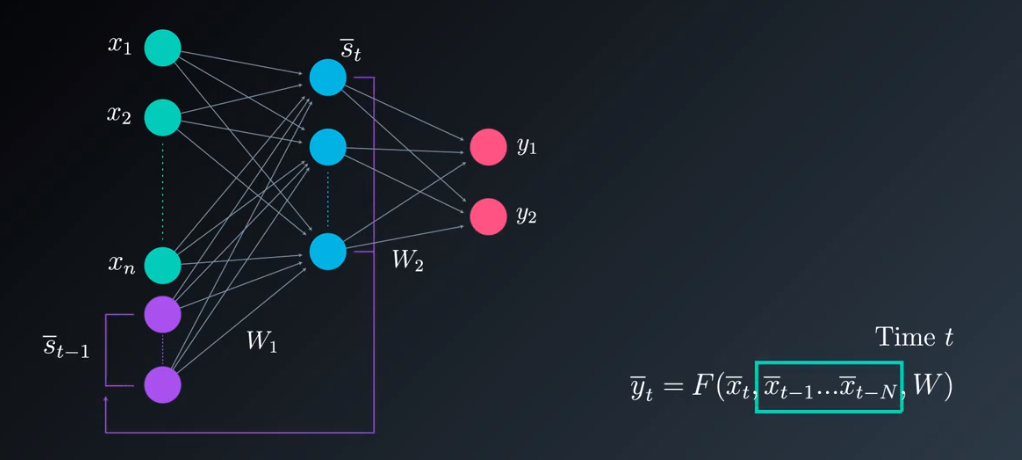
\includegraphics[width=0.8\linewidth,keepaspectratio]{rnn28}

\tiny{(Ref: RNN - Udacity)}

\end{center}

RNN can be imagined to be a usual ANN, with additional nodes from next layer back into inputs.
\end{frame}



% %%%%%%%%%%%%%%%%%%%%%%%%%%%%%%%%%%%%%%%%%%%%%%%%%%%
% \begin{frame}[fragile] \frametitle{What is RNN?}

% \begin{center}
% \includegraphics[width=0.8\linewidth,keepaspectratio]{rnn23}
% \end{center}
% One-to-One: Vanilla mode of processing without RNN, from fixed-sized input to fixed-sized output (e.g. image classification).
% \end{frame}

% %%%%%%%%%%%%%%%%%%%%%%%%%%%%%%%%%%%%%%%%%%%%%%%%%%%
% \begin{frame}[fragile] \frametitle{What is RNN?}

% \begin{center}
% \includegraphics[width=0.8\linewidth,keepaspectratio]{rnn23}
% \end{center}
% One-to-Many: Sequence output (e.g. image captioning takes an image (fixed size) and outputs a sentence of words).
% \end{frame}


% %%%%%%%%%%%%%%%%%%%%%%%%%%%%%%%%%%%%%%%%%%%%%%%%%%%
% \begin{frame}[fragile] \frametitle{Recurrent neural networks}
% \begin{center}
% \includegraphics[width=0.8\linewidth,keepaspectratio]{rnn23}
% \end{center}
% Many-to-One: Sequence input (e.g. sentiment analysis where a given sentence is classified as expressing positive or negative sentiment).
% \end{frame}

% %%%%%%%%%%%%%%%%%%%%%%%%%%%%%%%%%%%%%%%%%%%%%%%%%%%
% \begin{frame}[fragile] \frametitle{Recurrent neural networks}
% \begin{center}
% \includegraphics[width=0.8\linewidth,keepaspectratio]{rnn23}
% \end{center}
% Many-to-Many: Sequence input and sequence output (e.g. Machine Translation: an RNN reads a sentence in English and then outputs a sentence in French).
% \end{frame}

% % %%%%%%%%%%%%%%%%%%%%%%%%%%%%%%%%%%%%%%%%%%%%%%%%%%%
% % \begin{frame}[fragile] \frametitle{Recurrent neural networks}
% % \begin{center}
% % \includegraphics[width=0.8\linewidth,keepaspectratio]{rnn23}
% % \end{center}
% % Many-to-Many: Synced sequence input and output (e.g. video classification where we wish to label each frame of the video).
% % \end{frame}

% %%%%%%%%%%%%%%%%%%%%%%%%%%%%%%%%%%%%%%%%%%%%%%%%%%%
% \begin{frame}[fragile] \frametitle{Recurrent neural networks}
% \begin{center}
% \includegraphics[width=0.8\linewidth,keepaspectratio]{rnn23}
% \end{center}
% Notice that in every case are no pre-specified constraints on the lengths sequences because the recurrent transformation (green) is fixed and can be applied as many times as we like.
% \end{frame}



% %%%%%%%%%%%%%%%%%%%%%%%%%%%%%%%%%%%%%%%%%%%%%%%%%%%
% \begin{frame}[fragile] \frametitle{RNN: Sequential processing in absence of sequences.}
% \begin{center}
% \includegraphics[width=0.3\linewidth,keepaspectratio]{rnn24}
% \end{center}
% Images are fixed size. But for sequential numbers in it, RNN learns to read out house numbers from left to right.
% \end{frame}


%% http://karpathy.github.io/2015/05/21/rnn-effectiveness/
%% https://www.youtube.com/watch?v=iX5V1WpxxkY&index=10&list=LLsBKTrp45lTfHa_p49I2AEQ








% %%%%%%%%%%%%%%%%%%%%%%%%%%%%%%%%%%%%%%%%%%%%%%%%%%%
% \begin{frame}[fragile] \frametitle{RNNs Intuition}

% \begin{itemize}
% \item Human thoughts have persistence; humans don't start their thinking from scratch every second. 
% \item As you read this sentence, you understand each word based on your understanding of previous words.  
% \end{itemize}
% \end{frame}

% %%%%%%%%%%%%%%%%%%%%%%%%%%%%%%%%%%%%%%%%%%%%%%%%%%%
% \begin{frame}[fragile] \frametitle{RNNs Intuition}

% \begin{itemize}
% \item One of the appeals of RNNs is the idea that they are able to connect previous information to the present task
% \item E.g., using previous video frames to inform the understanding of the present frame.
% \item E.g., a language model tries to predict the next word based on the previous ones.
% \end{itemize}
% \end{frame}

% %%%%%%%%%%%%%%%%%%%%%%%%%%%%%%%%%%%%%%%%%%%%%%%%%%%
% \begin{frame}[fragile] \frametitle{What is Neural Memory?}

% \begin{itemize}
% \item List the alphabet forward\ldots. you can do it, yes?
% \item List the alphabet backward\ldots. hmmm\ldots perhaps a bit tougher.
% \item Try with the lyrics of a song you know?
% \item Why is it easier to recall forward than it is to recall backward? Can you jump into the middle of the second verse?\ldots hmm\ldots also difficult. Why?
% \end{itemize}
% \end{frame}

% %%%%%%%%%%%%%%%%%%%%%%%%%%%%%%%%%%%%%%%%%%%%%%%%%%%
% \begin{frame}[fragile] \frametitle{What is Neural Memory?}

% \begin{itemize}
% \item There's a very logical reason for this
% \item You learned them as a sequence. 
% \item You are really good at indexing from one letter to the next.
% \item It's a kind of conditional memory. (Once you given a start of poem, you can recite it further)
% \item All these  tasks are easier when you know what happened earlier in the sequence
% \end{itemize}
% \end{frame}

% %%%%%%%%%%%%%%%%%%%%%%%%%%%%%%%%%%%%%%%%%%%%%%%%%%%
% \begin{frame}[fragile] \frametitle{What is Neural Memory?}

% \begin{itemize}
% \item However, it's not that you don't have the song in your memory except when you're singing it. 
% \item Instead, when you try to jump straight to the middle of the song, you simply have a hard time finding that representation in your brain (perhaps that set of neurons).
% \item It starts searching all over looking for the middle of the song, but it hasn't tried to look for it this way before, so it doesn't have a map to the location of the middle of the second verse.
% \end{itemize}
% \end{frame}

%%%%%%%%%%%%%%%%%%%%%%%%%%%%%%%%%%%%%%%%%%%%%%%%%%%
\begin{frame}
  \begin{center}
    {\Large Memory in RNN}
  \end{center}
\end{frame}


% %%%%%%%%%%%%%%%%%%%%%%%%%%%%%%%%%%%%%%%%%%%%%%%%%%%
% \begin{frame}[fragile] \frametitle{What is Neural Memory?}

% \begin{itemize}
% \item If you wanted to train a neural network to predict whats the next scene would be in the next frame, it would be really helpful to know where the scene was in the last frame! 
% \item Sequential data like this is why we build recurrent neural networks.
% \end{itemize}
% \end{frame}

%%%%%%%%%%%%%%%%%%%%%%%%%%%%%%%%%%%%%%%%%%%%%%%%%%%
\begin{frame}[fragile] \frametitle{What is Neural Memory?}

\begin{itemize}
\item Neural networks have hidden layers. Normally, the state of your hidden layer is based ONLY on your input data. 
\item So, normally a neural network's information flow would look like this:
$input \rightarrow hidden  \rightarrow  output$
\item This is straightforward. Certain types of input create certain types of hidden layers. 
\item Certain types of hidden layers create certain types of output layers. 
\item It's kind-of a closed system. Memory changes this. 
\end{itemize}
\end{frame}


%%%%%%%%%%%%%%%%%%%%%%%%%%%%%%%%%%%%%%%%%%%%%%%%%%%
\begin{frame}[fragile] \frametitle{What is Neural Memory?}
\begin{itemize}
\item Memory means that the hidden layer is a combination of your input data at the current time-step and the hidden layer of the previous timestep.
$ (input + prev\_hidden) \rightarrow hidden \rightarrow output$
\item Why the hidden layer? Well, we could technically do this. 
$(input + prev\_input) \rightarrow hidden \rightarrow output$
\end{itemize}

\begin{center}
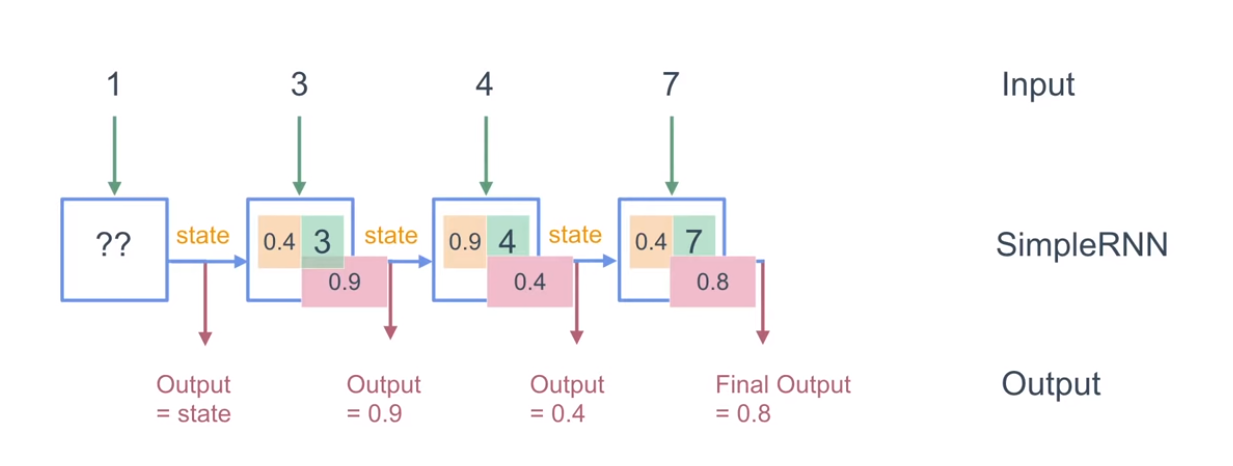
\includegraphics[width=0.8\linewidth,keepaspectratio]{rnn33}

{\tiny (Ref: Weights and Biases : Introduction to RNNs)}
\end{center}


\end{frame}

% %%%%%%%%%%%%%%%%%%%%%%%%%%%%%%%%%%%%%%%%%%%%%%%%%%%
% \begin{frame}[fragile] \frametitle{What is Neural Memory?}
% Here, we have 4 timesteps of a recurrent neural network pulling information from the previous hidden layer.
% \begin{itemize}
% \item $(input + empty\_hidden) \rightarrow hidden \rightarrow output$
% \item $(input + prev\_hidden) \rightarrow hidden \rightarrow output$
% \item $(input + prev\_hidden) \rightarrow hidden \rightarrow output$
% \item $(input + prev\_hidden) \rightarrow hidden \rightarrow output$
% \end{itemize}
% \end{frame}

%%%%%%%%%%%%%%%%%%%%%%%%%%%%%%%%%%%%%%%%%%%%%%%%%%%
\begin{frame}[fragile] \frametitle{What is Neural Memory?}
Each cell
\begin{itemize}
\item $h_t = tanh(W_{hh}h_{t-1} + W_{xh}X_t + b_h)$
\item $y_t = tanh(W_{hy}h_t + b_y)$
\item Back-propagation will adjust all the weights for all unrolled time-steps.
\end{itemize}


\begin{center}
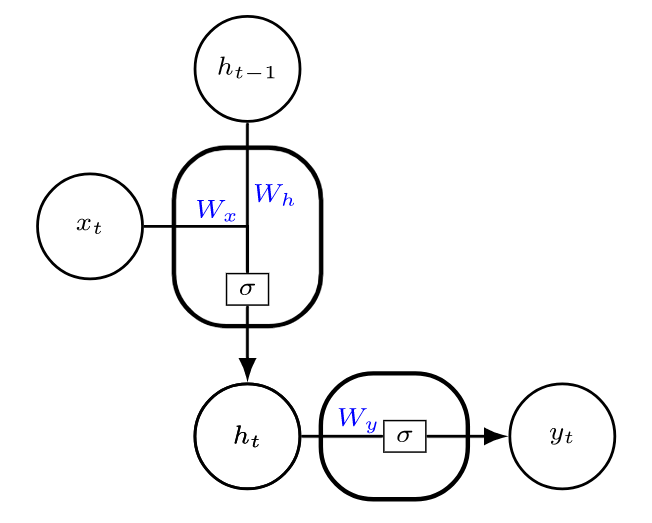
\includegraphics[width=0.3\linewidth,keepaspectratio]{rnn35}

{\tiny (Ref: RNN with Keras: Understanding computations - Alexis Huet)}


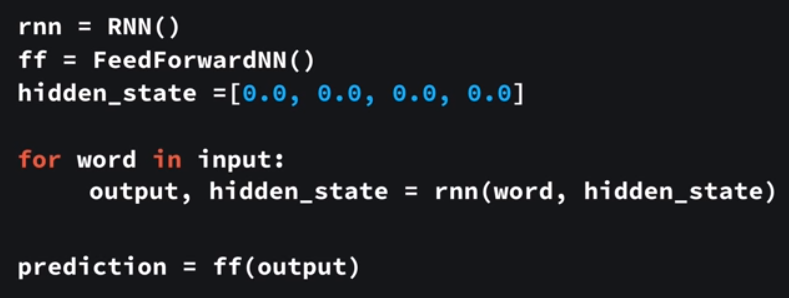
\includegraphics[width=0.6\linewidth,keepaspectratio]{rnn31}
\end{center}
\end{frame}


%%%%%%%%%%%%%%%%%%%%%%%%%%%%%%%%%%%%%%%%%%%%%%%%%%%
\begin{frame}[fragile] \frametitle{RNN with 2 hidden layers or units}
Each cell
\begin{itemize}
\item $h_t' = tanh(W_{hh}h_{t-1} + W_{xh}X_t + b_h)$
\item $h_t' = tanh(W_{hh}'h_{t-1}' + W_{xh}'X_t + b_h')$
\item $y_t = tanh(W_{hy}h_t' + b_y)$
\item Back-propagation will adjust all the weights for all unrolled time-steps.
\end{itemize}


\begin{center}
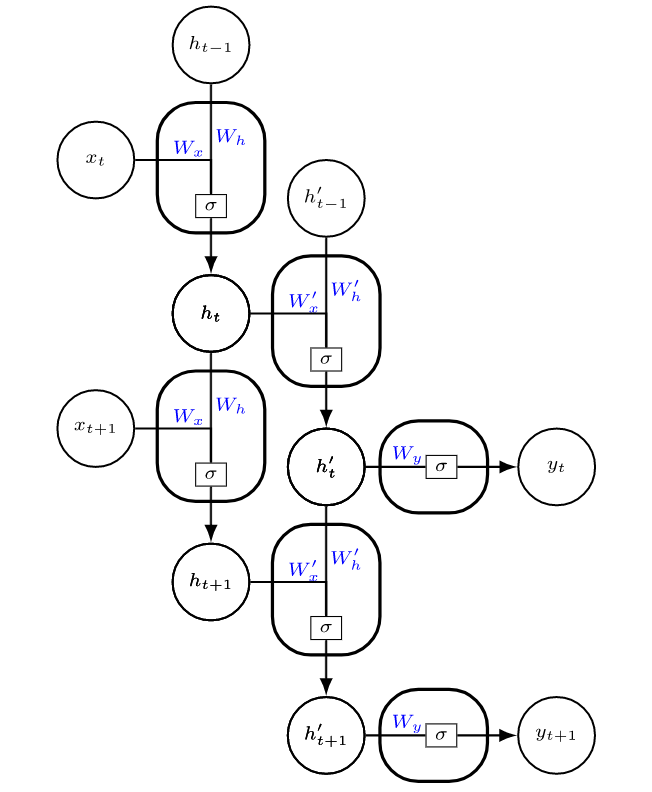
\includegraphics[width=0.3\linewidth,keepaspectratio]{rnn36}

{\tiny (Ref: RNN with Keras: Understanding computations - Alexis Huet)}
\end{center}
\end{frame}

%%%%%%%%%%%%%%%%%%%%%%%%%%%%%%%%%%%%%%%%%%%%%%%%%%%
\begin{frame}[fragile] \frametitle{GRU cell}
Each cell
\begin{align*}
z_t =& \sigma(W_{zx} x_t + W_{zh} h_{t-1} + b_z) \\
r_t =& \sigma(W_{rx} x_t + W_{rh} h_{t-1} + b_r) \\
\tilde{h}_t =& \tanh(W_{ox} x_t + W_{oh} r_t h_{t-1} + b_o) \\
 \\
h_t =& z_t h_{t-1} + (1 - z_t) \tilde{h}_t
\end{align*} %]]>


\begin{center}
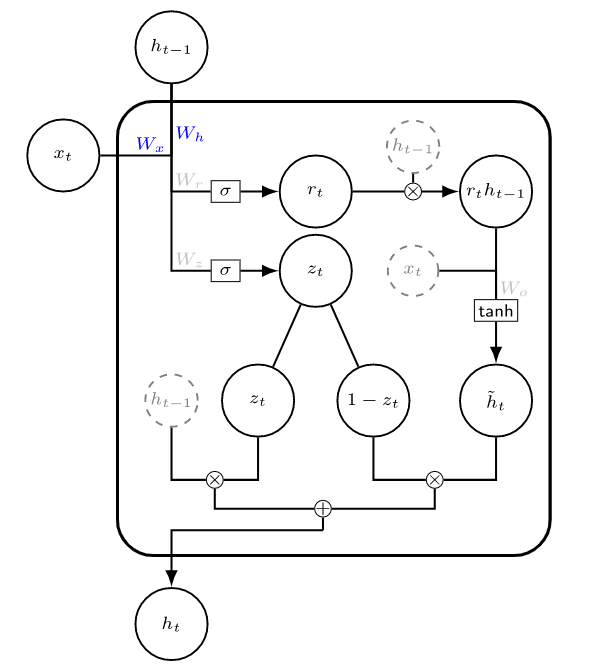
\includegraphics[width=0.3\linewidth,keepaspectratio]{rnn37}

{\tiny (Ref: RNN with Keras: Understanding computations - Alexis Huet)}
\end{center}
\end{frame}

%%%%%%%%%%%%%%%%%%%%%%%%%%%%%%%%%%%%%%%%%%%%%%%%%%%
\begin{frame}[fragile] \frametitle{LSTM cell}
Each cell
% <![CDATA[
\begin{align*}
i_t =& \sigma(W_{ix} x_t + W_{ih} h_{t-1} + b_i) \\
f_t =& \sigma(W_{fx} x_t + W_{fh} h_{t-1} + b_f) \\
\tilde{c}_t =& \tanh(W_{cx} x_t + W_{ch} h_{t-1} + b_c) \\
o_t =& \sigma(W_{ox} x_t + W_{oh} h_{t-1} + b_o) \\
 \\
c_t =& f_t c_{t-1} + i_t \tilde{c}_t \\
h_t =& o_t \tanh(c_t)
\end{align*} %]]>


\begin{center}
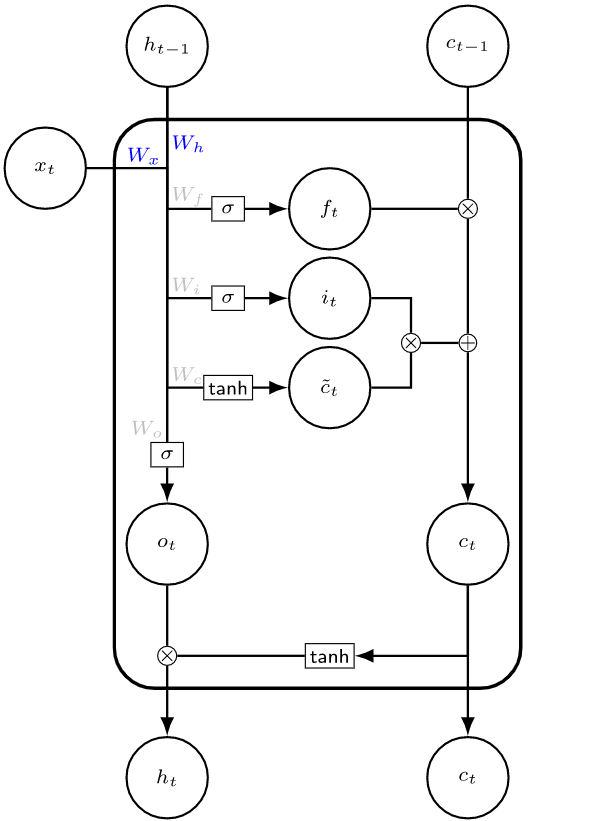
\includegraphics[width=0.2\linewidth,keepaspectratio]{rnn38}

{\tiny (Ref: RNN with Keras: Understanding computations - Alexis Huet)}
\end{center}
\end{frame}


% %%%%%%%%%%%%%%%%%%%%%%%%%%%%%%%%%%%%%%%%%%%%%%%%%%%
% \begin{frame}[fragile] \frametitle{What is Neural Memory?}
% Colored show how hidden layer gets updated. 
% 4 timesteps with hidden layer recurrence:
% \begin{center}
% \includegraphics[width=0.6\linewidth,keepaspectratio]{rnn1}
% \end{center}
% 4 timesteps with input  layer recurrence:
% \begin{center}
% \includegraphics[width=0.6\linewidth,keepaspectratio]{rnn2}
% \end{center}
% Focus on the last hidden layer (4th line).
% \end{frame}

% %%%%%%%%%%%%%%%%%%%%%%%%%%%%%%%%%%%%%%%%%%%%%%%%%%%
% \begin{frame}[fragile] \frametitle{What is Neural Memory?}
% \begin{itemize}
% \item  In the hidden layer recurrence, we see a presence of every input seen so far. In the input layer recurrence, it's exclusively defined by the current and previous inputs. 
% \item This is why we model hidden recurrence.
% \item Hidden recurrence learns what to remember whereas input recurrence is hard wired to just remember the immediately previous datapoint. 
% \end{itemize}
% \end{frame}

% %%%%%%%%%%%%%%%%%%%%%%%%%%%%%%%%%%%%%%%%%%%%%%%%%%%
% \begin{frame}[fragile] \frametitle{What is Neural Memory?}
% \begin{itemize}
% \item  Now compare and contrast these two approaches with the backwards alphabet and middle-of-song exercises. 
% \item The hidden layer is constantly changing as it gets more inputs. 
% \item Furthermore, the only way that we could reach these hidden states is with the correct sequence of inputs.
% \end{itemize}
% \end{frame}



% %%%%%%%%%%%%%%%%%%%%%%%%%%%%%%%%%%%%%%%%%%%%%%%%%%%
% \begin{frame}[fragile] \frametitle{What is Neural Memory?}
% \begin{itemize}
% \item  What's the practical difference? Let's say we were trying to predict the next word in a song given the previous. 
% \item The ``input layer recurrence'' would break down if the song accidentally had the same sequence of two words in multiple places. 
% \item Think about it, if the song had the statements ''I love you'', and ''I love carrots'', and the network was trying to predict the next word, how would it know what follows ''I love''? 
% It could be carrots. It could be you. The network REALLY needs to know more about what part of the song its in.
% \end{itemize}
% \end{frame}


% %%%%%%%%%%%%%%%%%%%%%%%%%%%%%%%%%%%%%%%%%%%%%%%%%%%
% \begin{frame}[fragile] \frametitle{What is Neural Memory?}
% \begin{itemize}
% \item  It could be carrots. 
% \item It could be you. 
% \item The network REALLY needs to know more about what part of the song its in.
% \item However, the ''hidden layer recurrence'' doesn't break down in this way. 
% \item It subtely remembers everything it saw (with memories becoming more subtle as it they fade into the past).
% \end{itemize}
% \end{frame}


% %%%%%%%%%%%%%%%%%%%%%%%%%%%%%%%%%%%%%%%%%%%%%%%%%%%
% \begin{frame}[fragile] \frametitle{RNN - Neural Network Memory}
% Normal NN process:
% \begin{itemize}
% \item Our input layer to the neural network is determined by our input dataset. 
% \item Each row of input data is used to generate the hidden layer (via forward propagation). 
% \item Each hidden layer is then used to populate the output layer (assuming only 1 hidden layer)
% \end{itemize}
% \end{frame}


% %%%%%%%%%%%%%%%%%%%%%%%%%%%%%%%%%%%%%%%%%%%%%%%%%%%
% \begin{frame}[fragile] \frametitle{RNN - Neural Network Memory}
% \begin{itemize}
% \item Just saw, memory means that the hidden layer is a combination of the input data and the previous hidden layer. 
% \item How is this done?
% \item Much like every other propagation in neural networks, it's done with a matrix. 
% \item This matrix defines the relationship between the previous hidden layer and the current one.
% \end{itemize}
% \end{frame}

% %%%
% %%%%%%%%%%%%%%%%%%%%%%%%%%%%%%%%%%%%%%%%%%%%%%%%%%%%%%
% %%%\begin{frame}[fragile] \frametitle{RNN - Neural Network Memory}
% %%%\begin{center}
% %%%\includegraphics[width=0.6\linewidth,keepaspectratio]{rnn3}
% %%%\end{center}
% %%%\begin{itemize}
% %%%\item SYNAPSE\_0 propagates the input data to the hidden layer. 
% %%%\item SYNAPSE\_1 propagates the hidden layer to the output data. 
% %%%\item The new matrix (SYNAPSE\_h, the recurrent one), propagates from the hidden layer (layer\_1) to the hidden layer at the next timestep (still layer\_1). 
% %%%\end{itemize}
% %%%\end{frame}

% %%%%%%%%%%%%%%%%%%%%%%%%%%%%%%%%%%%%%%%%%%%%%%%%%%%
% \begin{frame}
  % \begin{center}
    % {\Large Graphical view of RNN}
  % \end{center}
% \end{frame}


% %%%%%%%%%%%%%%%%%%%%%%%%%%%%%%%%%%%%%%%%%%%%%%%%%%%
% \begin{frame}[fragile] \frametitle{RNN in Steps}
% \begin{center}
% \includegraphics[width=0.6\linewidth,keepaspectratio]{rnn4}
% \end{center}
% \begin{itemize}
% \item It depicts 4 timesteps. 
% \item The first is exclusively influenced by the input data. 
% \item The second one is a mixture of the first and second inputs. 
% \item This continues on. 
% \end{itemize}
% \end{frame}

% %%%%%%%%%%%%%%%%%%%%%%%%%%%%%%%%%%%%%%%%%%%%%%%%%%%
% \begin{frame}[fragile] \frametitle{RNN in Steps}
% \begin{center}
% \includegraphics[width=0.6\linewidth,keepaspectratio]{rnn4}
% \end{center}
% \begin{itemize}
% \item You should recognize that, in some way, network 4 is ''full''. 
% \item Presumably, timestep 5 would have to choose which memories to keep and which ones to overwrite. 
% \item It's the notion of memory ''capacity''. As you might expect, bigger layers can hold more memories for a longer period of time.
% \end{itemize}
% \end{frame}

% %%%%%%%%%%%%%%%%%%%%%%%%%%%%%%%%%%%%%%%%%%%%%%%%%%%
% \begin{frame}[fragile] \frametitle{RNN in Steps}
% \begin{center}
% \includegraphics[width=0.6\linewidth,keepaspectratio]{rnn4}
% \end{center}
% \begin{itemize}
% \item Also, this is when the network learns to forget irrelevant memories and remember important memories. 
% \item What significant thing do you notice in timestep 3? 
% \item Why is there more green in the hidden layer than the other colors?
% \end{itemize}
% \end{frame}

% %%%%%%%%%%%%%%%%%%%%%%%%%%%%%%%%%%%%%%%%%%%%%%%%%%%
% \begin{frame}[fragile] \frametitle{RNN in Steps}
% \begin{itemize}
% \item Also notice that the hidden layer is the barrier between the input and the output. 
% \item In reality, the output is no longer a pure function of the input. 
% \item The input is just changing what's in the memory, 
% \item and the output is exclusively based on the memory. 
% \end{itemize}
% \end{frame}

% %%%%%%%%%%%%%%%%%%%%%%%%%%%%%%%%%%%%%%%%%%%%%%%%%%%
% \begin{frame}[fragile] \frametitle{RNN in Steps}
% \begin{center}
% \includegraphics[width=0.6\linewidth,keepaspectratio]{rnn4}
% \end{center}
% \begin{itemize}
% \item Another interesting takeaway. 
% \item If there was no input at timesteps 2,3,and 4, the hidden layer would still change from timestep to timestep. 
% \end{itemize}
% \end{frame}

% %%%%%%%%%%%%%%%%%%%%%%%%%%%%%%%%%%%%%%%%%%%%%%%%%%%
% \begin{frame}[fragile] \frametitle{RNN in Steps}

% Back-propagation Through Time

% \begin{center}
% \includegraphics[width=0.6\linewidth,keepaspectratio]{rnn5}
% \end{center}
% \begin{itemize}
% \item So, how do recurrent neural networks learn? 
% \item Errors are bright yellow, derivatives are mustard colored.
% \item Picture shows back propagation coming from 4th step upto 3rd.
% \end{itemize}
% \end{frame}

% %%%%%%%%%%%%%%%%%%%%%%%%%%%%%%%%%%%%%%%%%%%%%%%%%%%
% \begin{frame}[fragile] \frametitle{RNN in Steps}
% \begin{center}
% \includegraphics[width=0.6\linewidth,keepaspectratio]{rnn5}
% \end{center}
% \begin{itemize}
% \item They learn by fully propagating forward from 1 to 4 and then back-propagating all the derivatives from 4 back to 1. 
% \item Its normal neural network, except that we're re-using the same weights (synapses 0,1,and h) in their respective places. 
% \end{itemize}
% \end{frame}


%%%%%%%%%%%%%%%%%%%%%%%%%%%%%%%%%%%%%%%%%%%%%%%%%%%%%
%%\begin{frame}[fragile] \frametitle{Recurrent neural networks}
%%
%%\begin{itemize}
%%\item Recurrent Neural Networks are networks with loops in them, allowing information to persist.
%%\item In the above diagram, a chunk of neural network, A, looks at some input xt and outputs a value ht. 
%%\item A loop allows information to be passed from one step of the network to the next. 
%%\end{itemize}
%%\end{frame}


%%%%%%%%%%%%%%%%%%%%%%%%%%%%%%%%%%%%%%%%%%%%%%%%%%%
\begin{frame}
  \begin{center}
    {\Large Implementation of RNN}
  \end{center}
\end{frame}

%%%%%%%%%%%%%%%%%%%%%%%%%%%%%%%%%%%%%%%%%%%%%%%%%%%
\begin{frame}[fragile] \frametitle{RNN Inputs Specification}
FIXED sequence length case: Say,
\begin{itemize}
\item Dataset has 10000 rows and 64 features/columns
\item Need to generate classification model, binary, so labels are 0 or 1.
\item How does RNN handle this matrix (i.e., (1000,64))? Does it input each column something like this figure?
\item Should SimpleRNN() units always be equal to the number of features?
\end{itemize}

\begin{center}
\includegraphics[width=0.2\linewidth,keepaspectratio]{rnn32}
\end{center}


\end{frame}

%%%%%%%%%%%%%%%%%%%%%%%%%%%%%%%%%%%%%%%%%%%%%%%%%%%
\begin{frame}[fragile] \frametitle{RNN Inputs Specification}
\begin{itemize}
\item batch\_input\_shape to be with shape: \lstinline|(batch_size, X.shape[1], 1)|
\item So batch size* 1000 examples will go at a time. Total, 10 such batches.
\item Each of the 1000 example contains \lstinline|X.shape[1]| time-stamps (number of pink boxes in your image, same as number of features, ie 64) and each time-stamp is shape 1 (scalar). Dimensionality of that entity is 1. It can be a vector as well.
\item So input shape is \lstinline|(1000,64,1)|
\item The larger a batch, the more representative the computed gradient is for the whole data set, but larger memory requirements
\end{itemize}

{\tiny (More info: https://stats.stackexchange.com/questions/153531/what-is-batch-size-in-neural-network)}

\end{frame}

%%%%%%%%%%%%%%%%%%%%%%%%%%%%%%%%%%%%%%%%%%%%%%%%%%%
\begin{frame}[fragile] \frametitle{RNN Inputs Specification: Batch Size, Num Steps}
\begin{itemize}
\item `batch size' pertains to the amount of training samples to consider at a time for updating your network weights. Training can be erratic if weights are updated for each row. After a training pass of size batch\_size, the gradient of your loss function with respect to each of the network parameters is computed and your weights updated.
\item Till the batch is over, losses per training sample are either averaged or accumulated, with that values, weights are updated. {\tiny (Ref: https://stats.stackexchange.com/questions/174708/how-are-weights-updated-in-the-batch-learning-method-in-neural-networks)}

\item In RNN, it is computationally very, very expensive to calculate the gradients of the loss function with respect to network parameters if you have to consider back-propagation through all states since the creation of your network, there is a neat little trick to speed up your computation: approximate your gradients with a subset of historical network states num\_steps.
\end{itemize}

*
% \begin{center}
% \includegraphics[width=0.2\linewidth,keepaspectratio]{rnn32}
% \end{center}

{\tiny (More info: https://stackoverflow.com/questions/44381450/doubts-regarding-batch-size-and-time-steps-in-rnn)}

\end{frame}


%%%%%%%%%%%%%%%%%%%%%%%%%%%%%%%%%%%%%%%%%%%%%%%%%%%
\begin{frame}[fragile] \frametitle{RNN Inputs Specification: Batch Size, Num Steps}
Example: data size of 100; batch size of 5, for 30 network parameter updates during each epoch. 
\begin{itemize}
\item Propagates the first 5 training examples, updates its parameters based on the optimization method provided, then takes the next 5, until it made a full pass over the data. 
\item num\_steps determines the amount of cells you unroll and hence the amount of data used in gradient computation. 
\item As each cell/layer shares parameters, this does not result in an increase in parameters to optimize, but it enables context learning, which is why you'd want RNNs in the first place
\end{itemize}
So, NUM STEPS is the number of `features' you LOOK BACK (in case of text-words input) or consider while computing gradients and updating the weights.

*
% \begin{center}
% \includegraphics[width=0.2\linewidth,keepaspectratio]{rnn32}
% \end{center}

{\tiny (More info: https://stackoverflow.com/questions/44381450/doubts-regarding-batch-size-and-time-steps-in-rnn)}

\end{frame}


%%%%%%%%%%%%%%%%%%%%%%%%%%%%%%%%%%%%%%%%%%%%%%%%%%%
\begin{frame}[fragile] \frametitle{RNN LAYER Specification}
RNN Layer can have multiple hidden states, physically but internally to the cell. Each physical RNN cell (called units) unrolls time-step wise.

\begin{itemize}
\item Do we have to have RNN units, ie green, boxes, sames as number of columns or features, ie 64. %Green boxes are just time-step wise rolling, ie looping.
\item No! units will be your output dim. Thats inside direction, its about number of internal state values, which are given as outputs as well as hidden states passed to the next time-step.
\item This is '\ldots to MANY" architecture, for predicting next $n$ outputs.
\item Units will be the shape of the RNN's internal states. 
% \item So, if you declare units=2000 your output will be (1000,2000).)
% \item Each weight matrix will be num features x num outputs.
% \item Each output will get tuned, optimized as per its given output label.
% \item More units, is better to model the function. In case you want singular output you can still have more units and then later, add a dense layer to reduce the dimension to 1.
\end{itemize}

\begin{center}
\includegraphics[width=0.8\linewidth,keepaspectratio]{rnn34}

{\tiny (Ref: Weights and Biases : Introduction to RNNs)}

\end{center}


\end{frame}

%%%%%%%%%%%%%%%%%%%%%%%%%%%%%%%%%%%%%%%%%%%%%%%%%%%
\begin{frame}[fragile] \frametitle{RNN LAYER Specification}
RNN Layer can have multiple hidden states, physically but internally to the cell. Each physical RNN cell (called units) unrolls time-step wise.

\begin{itemize}
% \item Do we have to have RNN units, ie green, boxes, sames as number of columns or features, ie 64. %Green boxes are just time-step wise rolling, ie looping.
% \item No! units will be your output dim. Thats inside direction, its about number of internal state values, which are given as outputs as well as hidden states passed to the next time-step.
% \item This is '\ldots to MANY" architecture, for predicting next $n$ outputs.
% \item Units will be the shape of the RNN's internal states. 
\item So, if you declare units=2000 your output will be (1000,2000).)
\item Each weight matrix will be num features x num outputs.
\item Each output will get tuned, optimized as per its given output label.
\item More units, is better to model the function. In case you want singular output you can still have more units and then later, add a dense layer to reduce the dimension to 1.
\end{itemize}

\begin{center}
\includegraphics[width=0.8\linewidth,keepaspectratio]{rnn34}

{\tiny (Ref: Weights and Biases : Introduction to RNNs)}

\end{center}


\end{frame}


%%%%%%%%%%%%%%%%%%%%%%%%%%%%%%%%%%%%%%%%%%%%%%%%%%%
\begin{frame}[fragile] \frametitle{RNN Inputs Specification}
VARIABLE sequence length case: Say,
\begin{itemize}
\item Can either PAD the sequence with '0's and make it FIXED size, for each batch (or overall), else specify 'None' for that variable for time steps in Keras.  If you don't want `0' padding, then you can specify sample weights. 
\item Now, suppose length of training examples in
\begin{align*}
batch-1 &= 10, \\
batch-2 &= 15. \\
batch-3 &= 18 \ldots
\end{align*}
\item Now while training batch-1 , RNN will be unrolled/looped 10 times. For batch-2, 15 times and so on. The number of weights do not change, or even the network architecture does not change, but just the times same architecture is looped, changes in each batch.
\end{itemize}

{\tiny (Ref: https://datascience.stackexchange.com/questions/26366/training-an-rnn-with-examples-of-different-lengths-in-keras)}.


\end{frame}


%%%%%%%%%%%%%%%%%%%%%%%%%%%%%%%%%%%%%%%%%%%%%%%%%%%
\begin{frame}[fragile] \frametitle{RNN Inputs Specification}
\begin{itemize}

\item But, within a batch, do we need same fixed length of all sequences?
\item Because Tensorflow (or any other framework) works on tensors/arrays and those can't be "ragged" like $[[1,2,3],[4,5]]$. 
\item They need to be rectangular. Thats why within a batch, it needs to be fixed size. 
\item Anyway achieved by num steps parameter, it extends or truncates. 
\item The reason a fixed length is used in keras, is because it greatly improves performance by creating tensors of fixed shapes. 
\item But that's only for training. After training, you'll have learned the right weights for your task.
\end{itemize}

{\tiny (Ref: https://datascience.stackexchange.com/questions/26366/training-an-rnn-with-examples-of-different-lengths-in-keras)}.
% \begin{center}
% \includegraphics[width=0.2\linewidth,keepaspectratio]{rnn32}
% \end{center}


\end{frame}


%%%%%%%%%%%%%%%%%%%%%%%%%%%%%%%%%%%%%%%%%%%%%%%%%%%
\begin{frame}[fragile] \frametitle{RNN Model}
Code: 
\begin{lstlisting}
X = X.reshape((X.shape[0], X.shape[1], 1)) # IT HAS TO BE 3D, so fake 1 dim added
tr_X, ts_X, tr_y, ts_y = train_test_split(X, y, train_size=.8)
batch_size = 1000

model = Sequential()
model.add(SimpleRNN(64, activation='relu', batch_input_shape=(batch_size, X.shape[1], 1)))
model.add(Dense(1, activation='relu'))

model.compile(loss='binary_crossentropy', optimizer='adam', metrics=['accuracy'])

model.fit(tr_X, tr_y,
          batch_size=batch_size, epochs=1,
          shuffle=True, validation_data=(ts_X, ts_y))
\end{lstlisting}



\end{frame}

%%%%%%%%%%%%%%%%%%%%%%%%%%%%%%%%%%%%%%%%%%%%%%%%%%%
\begin{frame}[fragile] \frametitle{RNN Parameters calculations}

\begin{itemize}
\item num\_units = equals the number of units in the RNN
\item num\_features = equals the number features of your input
\item input\_weights = num\_features*num\_units
\item recurrent\_weights = num\_units*num\_units
\item biases = num\_units*1
\item total params = recurrent\_weights + input\_weights + biases
\end{itemize}

% \begin{center}
% \includegraphics[width=0.2\linewidth,keepaspectratio]{rnn32}
% \end{center}


\end{frame}

%%%%%%%%%%%%%%%%%%%%%%%%%%%%%%%%%%%%%%%%%%%%%%%%%%%
\begin{frame}[fragile] \frametitle{RNNs Model Summary}
\begin{lstlisting}
Layer (type)                 Output Shape              Param #   
=================================================================
simple_rnn_1 (SimpleRNN)     (1000, 64)                4224      
_________________________________________________________________
dense_1 (Dense)              (1000, 1)                 65        
=================================================================
Total params: 4,289
Trainable params: 4,289
Non-trainable params: 0
_________________________________________________________________
\end{lstlisting}


% \begin{center}
% \includegraphics[width=0.2\linewidth,keepaspectratio]{rnn32}
% \end{center}


\end{frame}





%%%%%%%%%%%%%%%%%%%%%%%%%%%%%%%%%%%%%%%%%%%%%%%%%%%
\begin{frame}
  \begin{center}
    {\Large Conclusions}
  \end{center}
\end{frame}


%%%%%%%%%%%%%%%%%%%%%%%%%%%%%%%%%%%%%%%%%%%%%%%%%%%
\begin{frame}[fragile] \frametitle{RNNs advantages}

\begin{itemize}
\item The applications of standard Neural Networks (and also Convolutional Networks) are limited due to:
\item They only accepted a fixed-size vector as input (e.g., an image) and produce a fixed-size vector as output (e.g., probabilities of different classes). 
\item These models use a fixed amount of computational steps (e.g. the number of layers in the model).
\end{itemize}
\end{frame}


%%%%%%%%%%%%%%%%%%%%%%%%%%%%%%%%%%%%%%%%%%%%%%%%%%%
\begin{frame}[fragile] \frametitle{RNNs advantages}

\begin{itemize}
\item Recurrent Neural Networks are unique as they allow us to operate over sequences of vectors.
\item Sequences in the input, the output, or in the most general case both
\end{itemize}
\end{frame}


%%%
%%%
%%%
%%%
%%%%%%%%%%%%%%%%%%%%%%%%%%%%%%%%%%%%%%%%%%%%%%%%%%%%%%
%%%\begin{frame}[fragile] \frametitle{Stateful models}
%%%
%%%
%%%\begin{itemize}
%%%\item Using this idea, we can think of variable width inputs
%%%such that each new word simply updates our current prediction.
%%%In this way an RNN has two types of data inside of it:
%%%\begin{itemize}
%%%\item fixed weights, just as we have been using with CNNs
%%%\item stateful variables that are updated as it observes words
%%%in a document
%%%\end{itemize}
%%%\item Can also think of this as giving `memory' to the neural
%%%network.
%%%\end{itemize}
%%%\end{frame}
%%%
%%%
%%%
%%%%%%%%%%%%%%%%%%%%%%%%%%%%%%%%%%%%%%%%%%%%%%%%%%%%%%
%%%\begin{frame}[fragile] \frametitle{RNNs Memory}
%%%\begin{center}
%%%\includegraphics[width=0.8\linewidth,keepaspectratio]{rnnmem}
%%%\end{center}
%%%\end{frame}
%%%
%%%
%%%
%%%%%%%%%%%%%%%%%%%%%%%%%%%%%%%%%%%%%%%%%%%%%%%%%%%%%%
%%%\begin{frame}[fragile] \frametitle{}
%%%
%%%
%%%
%%%A third way of thinking about recurrent neural networks is to
%%%think of a network that has a loop in it. However, the self-input
%%%get's applied the \textit{next} time it is called.
%%%
%%%\begin{center}
%%%\includegraphics[width=0.3\linewidth,keepaspectratio]{cloah01.png}
%%%\end{center}
%%%
%%%\end{frame}
%%%
%%%%%%%%%%%%%%%%%%%%%%%%%%%%%%%%%%%%%%%%%%%%%%%%%%%%%%
%%%\begin{frame}[fragile] \frametitle{}
%%%
%%%A fourth way of thinking about a recurrent neural network is
%%%mathematically. We now have two parts to the update function
%%%in the RNN:
%%%\begin{align*}
%%%h_{t} &= {W x_t + b} + {U h_{t-1}}
%%%\end{align*}
%%%Notice that $U$ must always be a square matrix,
%%%because we could unravel this one time further to yield:
%%%\begin{align*}
%%%h_{t} &= W x_t + b + U W x_{t-1} + U b + U^2 h_{t-2}
%%%\end{align*}
%%%
%%%\end{frame}
%%%
%%%%%%%%%%%%%%%%%%%%%%%%%%%%%%%%%%%%%%%%%%%%%%%%%%%%%%
%%%\begin{frame}[fragile] \frametitle{What's different?}
%%%\begin{itemize}
%%%\item At each time step, output of hidden layers $H$ are added back for the next input.
%%%\item Outputs are also calculated at each time step ($Y_t$)
%%%\item Same wts and biases are shared across iterations
%%%\item Its like a state machine cell (remembering something)
%%%\item Can be used for sequences
%%%\end{itemize}
%%%
%%%
%%%\end{frame}
%%%
%%%%%%%%%%%%%%%%%%%%%%%%%%%%%%%%%%%%%%%%%%%%%%%%%%%%%%
%%%\begin{frame}[fragile] \frametitle{What's different?}
%%%\begin{center}
%%%\includegraphics[width=0.8\linewidth,keepaspectratio]{rnnwts}
%%%\end{center}
%%%
%%%\end{frame}
%%%
%%%
%%%
%%%%%%%%%%%%%%%%%%%%%%%%%%%%%%%%%%%%%%%%%%%%%%%%%%%%%%
%%%\begin{frame}[fragile] \frametitle{RNN}
%%%
%%%\begin{center}
%%%\includegraphics[width=0.8\linewidth,keepaspectratio]{rnnsamewts}
%%%\end{center}
%%%Output $y^i$ depends on $x_1, x_2,\ldots x_i$
%%%
%%%\end{frame}
%%%
%%%%%%%%%%%%%%%%%%%%%%%%%%%%%%%%%%%%%%%%%%%%%%%%%%%%%%
%%%\begin{frame}[fragile] \frametitle{On Sequences}
%%%
%%%
%%%\begin{itemize}
%%%\item Each cell, gets input, does iterations to try to match with given outputs. In the process, calculates wts and biases, as usual. May not work. 
%%%\item Instead of one cell, have a series and see if $Y_5$ can be forced.
%%%\item It is achieved by backpropagating through all cells, backwards.
%%%\item All $H$''s are adjusted, so $W$''s and $b$''s
%%%\item Can train on sequence of characters and verify open and close brackets
%%%\end{itemize}
%%%\begin{center}
%%%\includegraphics[width=0.8\linewidth,keepaspectratio]{rnnseq}
%%%\end{center}
%%%
%%%\end{frame}
%%%
%%%%%%%%%%%%%%%%%%%%%%%%%%%%%%%%%%%%%%%%%%%%%%%%%%%%%%
%%%\begin{frame}[fragile] \frametitle{How to train RNN?}
%%%
%%%\begin{center}
%%%\includegraphics[width=0.8\linewidth,keepaspectratio]{rnntrain}
%%%\end{center}
%%%Find the network parameters to minimize the total cost
%%%
%%%\end{frame}
%%%
%%%
%%%
%%%%%%%%%%%%%%%%%%%%%%%%%%%%%%%%%%%%%%%%%%%%%%%%%%%%%%
%%%\begin{frame}[fragile] \frametitle{Of course it can be deep}
%%%\begin{center}
%%%\includegraphics[width=0.8\linewidth,keepaspectratio]{rnndeep}
%%%\end{center}
%%%\end{frame}
%%%
%%%%%%%%%%%%%%%%%%%%%%%%%%%%%%%%%%%%%%%%%%%%%%%%%%%%%%
%%%\begin{frame}[fragile] \frametitle{Bidirectional RNN}
%%%\begin{center}
%%%\includegraphics[width=\linewidth,keepaspectratio]{rnnbi}
%%%\end{center}
%%%\end{frame}
%%%
%%%%%%%%%%%%%%%%%%%%%%%%%%%%%%%%%%%%%%%%%%%%%%%%%%%%%%
%%%\begin{frame}[fragile] \frametitle{Bidirectional RNN}
%%%\begin{center}
%%%\includegraphics[width=\linewidth,keepaspectratio]{rnnbi}
%%%\end{center}
%%%\end{frame}
%%%
%%%
%%%%%%%%%%%%%%%%%%%%%%%%%%%%%%%%%%%%%%%%%%%%%%%%%%%%%%
%%%\begin{frame}[fragile] \frametitle{Many to Many (Output is shorter)}
%%%Both input and output are both sequences, but the output is shorter.
%%%E.g. Speech Recognition
%%%\begin{center}
%%%\includegraphics[width=\linewidth,keepaspectratio]{rnnmm}
%%%\end{center}
%%%\end{frame}
%%%
%%%%%%%%%%%%%%%%%%%%%%%%%%%%%%%%%%%%%%%%%%%%%%%%%%%%%%
%%%\begin{frame}[fragile] \frametitle{Can also Stack them}
%%%\begin{center}
%%%\includegraphics[width=\linewidth,keepaspectratio]{rnnstack}
%%%\end{center}
%%%\end{frame}
%%%
%%%%%%%%%%%%%%%%%%%%%%%%%%%%%%%%%%%%%%%%%%%%%%%%%%%%%%
%%%\begin{frame}[fragile] \frametitle{RNN Types a summary}
%%%Input vectors are in red, output vectors are in blue and green vectors hold the RNN's state
%%%\begin{center}
%%%\includegraphics[width=\linewidth,keepaspectratio]{rnntypes}
%%%\end{center}
%%%
%%%\end{frame}
%%%
%%%%%%%%%%%%%%%%%%%%%%%%%%%%%%%%%%%%%%%%%%%%%%%%%%%%%%
%%%\begin{frame}[fragile] \frametitle{RNN Types a summary}
%%%\begin{itemize}
%%%\item Standard mode of processing without RNN, from fixed-sized input to fixed-sized output (e.g. image classification). 
%%%\item Sequence output (e.g. image captioning takes an image and outputs a sentence of words). 
%%%\item Sequence input (e.g. sentiment analysis where a given sentence is classified as expressing positive or negative sentiment). 
%%%\item Sequence input and sequence output (e.g. Machine Translation: an RNN reads a sentence in English and then outputs a sentence in French). 
%%%\item Synced sequence input and output (e.g. video classification where we wish to label each frame of the video).
%%%\end{itemize}
%%%\end{frame}
%%%
%%%%%%%%%%%%%%%%%%%%%%%%%%%%%%%%%%%%%%%%%%%%%%%%%%%%%%
%%%\begin{frame}[fragile] \frametitle{RNN Apps}
%%%\begin{center}
%%%\includegraphics[width=\linewidth,keepaspectratio]{rnnapps}
%%%\end{center}
%%%\end{frame}
%%%
%%%%%%%%%%%%%%%%%%%%%%%%%%%%%%%%%%%%%%%%%%%%%%%%%%%%%%
%%%\begin{frame}[fragile] \frametitle{Name Entity Recognition}
%%%Detecting named entities like name of people, locations, organization, etc. in a sentence.
%%%\begin{center}
%%%\includegraphics[width=\linewidth,keepaspectratio]{rnnner}
%%%\end{center}
%%%\end{frame}
%%%
%%%%%%%%%%%%%%%%%%%%%%%%%%%%%%%%%%%%%%%%%%%%%%%%%%%%%%
%%%\begin{frame}[fragile] \frametitle{Name Entity Recognition}
%%%\begin{center}
%%%\includegraphics[width=\linewidth,keepaspectratio]{rnnnerlayer}
%%%\end{center}
%%%\end{frame}
%%%
%%%%%%%%%%%%%%%%%%%%%%%%%%%%%%%%%%%%%%%%%%%%%%%%%%%%%%
%%%\begin{frame}[fragile] \frametitle{Unfortunately}
%%%RNN-based network is not always easy to learn
%%%\begin{center}
%%%\includegraphics[width=\linewidth,keepaspectratio]{rnndisadv}
%%%\end{center}
%%%\end{frame}
%%%
%%%%%%%%%%%%%%%%%%%%%%%%%%%%%%%%%%%%%%%%%%%%%%%%%%%%%%
%%%\begin{frame}[fragile] \frametitle{Errors}
%%%The error surface is rough.
%%%\begin{center}
%%%\includegraphics[width=\linewidth,keepaspectratio]{rnnerr}
%%%\end{center}
%%%\end{frame}
%%%
%%%
%%%%%%%%%%%%%%%%%%%%%%%%%%%%%%%%%%%%%%%%%%%%%%%%%%%%%%
%%%\begin{frame}[fragile] \frametitle{Anything better}
%%%\begin{itemize}
%%%\item ``Michael was born in Paris.<sentences> His mother tongue is ''
%%%\item Clue is far away. You need to have very long chain of such cells. That's limitation.
%%%\item Just few words is ok.
%%%\item Solution: LSTM (Long Short Term Memory)
%%%\end{itemize}
%%%\end{frame}
%%%
%%%
%%%%%%%%%%%%%%%%%%%%%%%%%%%%%%%%%%%%%%%%%%%%%%%%%%%%%%
%%%\begin{frame}[fragile] \frametitle{Anything better}
%%%\begin{center}
%%%\includegraphics[width=\linewidth,keepaspectratio]{rnn2lstm}
%%%\end{center}
%%%\end{frame}



% %%%%%%%%%%%%%%%%%%%%%%%%%%%%%%%%%%%%%%%%%%%%%%%%%%%
% \begin{frame}
  % \begin{center}
    % {\Large RNN variations}
    
    % LSTM-GRU
  % \end{center}
% \end{frame}

% %%%%%%%%%%%%%%%%%%%%%%%%%%%%%%%%%%%%%%%%%%%%%%%%%%%
% \begin{frame}[fragile] \frametitle{Recap: Simple RNN}
% \begin{center}
% \includegraphics[width=0.5\linewidth,keepaspectratio]{lstm49}

% \tiny{(Ref: Intro to Deep Learning - Coursera, National Research University Higher School of Economics)}
% \end{center}
% RNN takes previous hidden state ($h_{t-1}$), current input ($x_t$) and generates new/next hidden state ($h_t$) by formula $h_t = f_h ( Vx_t + Wh_{t-1} + b_h)$
% \end{frame}

%%%%%%%%%%%%%%%%%%%%%%%%%%%%%%%%%%%%%%%%%%%%%%%%%%%
\begin{frame}[fragile] \frametitle{RNN Shortcomings}
\begin{itemize}
\item RNN does not work in some situations
\item Especially when long past words need to be accounted for
\item Due to Vanishing Gradient problem.
\end{itemize}

\begin{center}
\includegraphics[width=\linewidth,keepaspectratio]{rnn42}
\end{center}
\end{frame}

%%%%%%%%%%%%%%%%%%%%%%%%%%%%%%%%%%%%%%%%%%%%%%%%%%%
\begin{frame}[fragile] \frametitle{RNN vanishing gradients}
\begin{itemize}
\item Vanilla RNNs suffers at vanishing gradients problems.
\item A modest recurrent neural network may have 200-to-400 input time steps, resulting conceptually in a very deep network.
\item problem: The derivative the activation nonlinearities, sigmoid or tanh, is smaller
than 1. So, after some timesteps, very minute gradient remains to make any weight changes. In further layers, weights do not change. So, NO TRAINING.
\item Solution: the hidden transfer function should be a linear function. Relu (rectilinear activation function) looks and acts like a linear function, making it easier to train and less likely to saturate, but is, in fact, a nonlinear function. The ReLU derivative is a constant of either 0 or 1, so it isn’t as likely to suffer from vanishing gradients.
\end{itemize}

\begin{center}
\includegraphics[width=0.8\linewidth,keepaspectratio]{rnn46}
\end{center}
\end{frame}

%%%%%%%%%%%%%%%%%%%%%%%%%%%%%%%%%%%%%%%%%%%%%%%%%%%
\begin{frame}[fragile] \frametitle{How LSTM solves Vanishing Gradient}
\begin{itemize}
\item LSTM increases memory network, handles more information, longer memory.
\item LSTM network has three gates that update and control the cell states.
\item So if we want Gradient not to vanish, our network needs to increase the likelihood that at least some of these sub gradients will not vanish.
\item Forget gate sub-gradient does not behave similarly with other sub-gradient, so they all do not converge to zero.
\end{itemize}

{\tiny (Ref: How LSTM networks solve the problem of vanishing gradients
- Nir Arbel)}

\end{frame}

%%%%%%%%%%%%%%%%%%%%%%%%%%%%%%%%%%%%%%%%%%%%%%%%%%%
\begin{frame}[fragile] \frametitle{Summary}
\begin{itemize}
\item RNNs suffer from vanishing gradients and caused by long series of multiplications of small values, diminishing the gradients and causing the learning process to become degenerate.
\item LSTMs solve the problem using a unique additive gradient structure that includes direct access to the forget gate’s activations, enabling the network to encourage desired behaviour from the error gradient using frequent gates update on every time step of the learning process.
\end{itemize}

{\tiny (Ref: How LSTM networks solve the problem of vanishing gradients
- Nir Arbel)}

\end{frame}

